\documentclass[12pt,aspectratio=169]{beamer}
\usepackage{fancyvrb}
\RecustomVerbatimCommand{\VerbatimInput}{VerbatimInput}{frame=single,
numbersep=1mm, numbers=left, formatcom=\color{orange}}
%\usepackage{kpfonts}
%\usepackage[bitstream-charter]{mathdesign}
\usepackage[utf8]{inputenc}
\usepackage{pgf}
\usepackage{verbatim}
%\usepackage{fontspec}
\usepackage[ruled,vlined,linesnumbered]{algorithm2e}
\IncMargin{1em}
\usetheme{Madrid}
\setbeamerfont{frametitle}{series=\bfseries}
\usecolortheme[dark]{solarized}
\setbeamertemplate{blocks}[rounded][shadow=false]
\setbeamertemplate{navigation symbols}{}


\author{Gianluca Della Vedova}
\title[Advanced Algorithms]{Advanced Techniques for Combinatorial Algorithms:
Fixed-Parameter Algorithms}
\institute[]{Univ. Milano--Bicocca\\
  \texttt{https://gianluca.dellavedova.org}}

\DeclareMathOperator{\poly}{\text{poly}}
\DeclareMathOperator{\polylog}{\text{polylog}}


% If you wish to uncover everything in a step-wise fashion, uncomment
% the following command:
% \beamerdefaultoverlayspecification{<+->}


\begin{document}

\begin{frame}
  \titlepage
\end{frame}


\begin{frame}\frametitle{Gianluca Della Vedova}
  \begin{itemize}
  \item
                Advanced Techniques for Combinatorial Algorithms
\item
{\small\url{https://gitlab.com/dellavg/advanced-algorithms}}
  \item
{\small\url{https://gianluca.dellavedova.org}}
  \item
{\small\url{gianluca.dellavedova@unimib.it}}
  \end{itemize}
\end{frame}

\begin{frame}\frametitle{Fixed-Parameter}
  \begin{itemize}
  \item
    An \textbf{NP}-hard problem does not go away
  \item
    Vertex cover
  \item
    Clique
  \item
    Independent set
  \item
    Dominating set
  \item
    Hamiltonian cycle
  \end{itemize}
\end{frame}

\begin{frame}\frametitle{Vertex Cover }
\begin{columns} 
  \begin{column}{0.48\textwidth}
  \begin{block}{Instance}
    Undirected graph $G=\langle V,E \rangle$, integer $k$.
  \end{block}
  \begin{block}{Question}
    Find a set $C\subset V$ such that for each edge $e\in E$ at least one endpoint of $e$
    belongs to $C$, and $|C|\le k$
  \end{block}
\end{column}
    
    \begin{column}{0.48\textwidth}
      \centering

  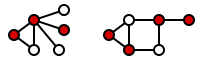
\includegraphics[height=0.2\textheight]{img/Vertex-cover}
\end{column}
\end{columns}
\end{frame}


\begin{frame}\frametitle{Clique }
\begin{columns} 
  \begin{column}{0.48\textwidth}
  \begin{block}{Instance}
    Undirected graph $G=\langle V,E \rangle$, integer $k$.
  \end{block}
  \begin{block}{Question}
    Find a set $C\subset V$ such that all pairs of vertices in $C$ are connected by an edge, and $|C|\ge k$
  \end{block}
\end{column}
    
    \begin{column}{0.48\textwidth}
      \centering

  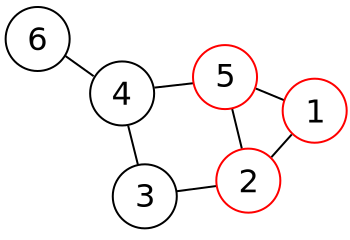
\includegraphics[height=0.5\textheight]{img/6n-graf-clique}
\end{column}
\end{columns}
\end{frame}

\begin{frame}\frametitle{Independent Set }
\begin{columns} 
  \begin{column}{0.48\textwidth}
  \begin{block}{Instance}
    Undirected graph $G=\langle V,E \rangle$, integer $k$.
  \end{block}
  \begin{block}{Question}
    Find a set $I\subset V$ such that no two vertices in $K$ are connected by an edge, and $|K|\ge k$
  \end{block}
\end{column}
    
    \begin{column}{0.48\textwidth}
      \centering
  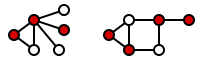
\includegraphics[height=0.2\textheight]{img/Vertex-cover}
\end{column}
\end{columns}
\end{frame}

\begin{frame}\frametitle{Dominating Set }
\begin{columns} 
  \begin{column}{0.48\textwidth}
  \begin{block}{Instance}
    Undirected graph $G=\langle V,E \rangle$, integer $k$.
  \end{block}
  \begin{block}{Question}
    Find a set $D\subset V$ such that for each vertex $v\notin D$, $v$ is adjacent to some
    $d\in D$, and $|D|\le k$
  \end{block}
\end{column}
    
    \begin{column}{0.48\textwidth}
      \centering
  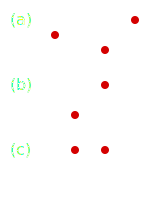
\includegraphics[height=0.7\textheight]{img/Dominating-set}
\end{column}
\end{columns}
\end{frame}



\begin{frame}\frametitle{Hamiltonian cycle}
\begin{columns} 
  \begin{column}{0.48\textwidth}
  \begin{block}{Instance}
    Undirected graph $G=\langle V,E \rangle$.
  \end{block}
  \begin{block}{Question}
    Find a cycle $C$ that visits each vertex  $v\in V$ exactly once.
%
  \end{block}
\end{column}
    \begin{column}{0.48\textwidth}
      \centering
  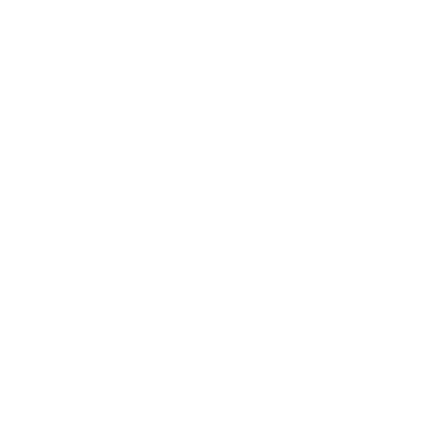
\includegraphics[height=0.7\textheight]{img/Grinberg_5CEC_Nonhamiltonian_graph}
\end{column}
\end{columns}
\end{frame}


\begin{frame}\frametitle{Longest Path}
\begin{columns} 
  \begin{column}{0.48\textwidth}
  \begin{block}{Instance}
    Undirected graph $G=\langle V,E \rangle$, integer $k$.
  \end{block}
  \begin{block}{Question}
    Find a simple (no vertex is visited twice) path $P$ of $G$, with $P$ consisting of $k$
    vertices.
%
  \end{block}
\end{column}
    \begin{column}{0.48\textwidth}
      \centering
  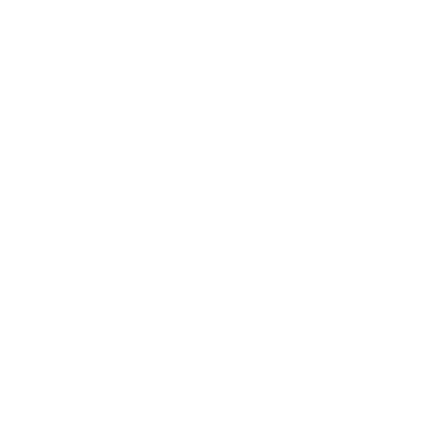
\includegraphics[height=0.7\textheight]{img/Grinberg_5CEC_Nonhamiltonian_graph}
\end{column}
\end{columns}
\end{frame}

\begin{frame}\frametitle{Fixed Parameter Tractable (FPT) }
  \begin{block}{FPT}
    Parameterized problem: pair $(I,k)$.
%
    The problem is in FPT if there is an algorithm with time $f(k)n^{\alpha}$, with
    $\alpha$ a constant and $f$ a function
  \end{block}

  \begin{block}{Typical times}
    \begin{itemize}
    \item
      $O(1.1^{k})n^{3}$
    \item
      $O(2^{k})n^{3}$
    \item
      $O(k^{k})n^{3}$
    \item
      $O(2^{k} + n^{3})$
    \item
      $(O(2^{2^{2^{...^{2}}}})n^{3})$
    \end{itemize}
  \end{block}
\end{frame} 

\begin{frame}\frametitle{Bounded Search Tree }
  The search tree has $O(f(k))n^{\alpha}$ nodes

  \begin{block}{Vertex Cover}
    Let $(u,v)\in E$.
%
    Then $u\in C$ or $v\in C$
  \end{block}

  \begin{itemize}
  \item
    How is the search tree?
  \item
    $2^{k}n$ time
  \end{itemize}
\end{frame} 

\begin{frame}\frametitle{Smaller Search Tree }
    \begin{block}{Proposition}
      Let $v$ be a node, let $N(v)$ be its neighbors.
%
      Then $v\in C$ or $N(v)\subseteq C$
    \end{block}
    \begin{block}{Proposition}
      No node has at least three neighbors.
%
      Then $G$ consists of vertex-disjoint cycle, and its smallest cover is trivial
    \end{block}

    \begin{block}{Corollary}
      Consider only vertices $v$ with $|N(v)|\ge 3$
    \end{block}
  \end{frame}

\begin{frame}\frametitle{Smaller Search Tree }
    \begin{block}{Two cases}
      \begin{enumerate}
      \item
        $v\in C$, then recurse on $G-v$ and height $k-1$
      \item
        $v\notin C$, then recurse on $G-N(v)$ and height at most $k-3$
      \end{enumerate}
    \end{block}

      \begin{enumerate}
      \item
    Number of nodes $f(k) = f(k-1) + f(k-3) +1$
  \item
    $f(k) \le 5^{\frac{k}{4}}< 1.5^{k}$
  \end{enumerate}
\end{frame}



\begin{frame}\frametitle{Reduction to a Kernel}
  \begin{enumerate}
  \item
    Find all vertices $L$ with degree $\ge k$.
%
    If $|L|>k$, then no cover of size $k$.
%
    Let $k_{1} = k - |L|$
  \item
    $G_{1} = G - L$.
%
    If $G_{1}$ has more than $k_{1}(k+1)$ vertices, then no cover of size $k$.
  \item
    Find  $k_{1}$-cover of $G_{1}$, time $O(n + k^{2k})$
  \item
    Improve to $O(n + 2^{k}k^{2})$
  \end{enumerate}
\end{frame}


\begin{frame}\frametitle{Color Coding }
  \begin{block}{Colorful Path}
    \begin{enumerate}
    \item
      Color each vertex with $k$ colors
    \item
      Colorful path: each vertex has a distinct color
    \end{enumerate}
  \end{block}

  \begin{block}{Random coloring}
    Probability that a path is colorful: $\frac{k!}{k^{k}} \ge e^{-k}$
  \end{block}

  \begin{block}{Dynamic programming}
    \begin{itemize}
      \item
        Given a coloring, find a colorful path (if it exists)
      \item
        Keep only the colors
      \item
        Time $(2^{O(k)}|E|)$
      \end{itemize}
    \end{block}
\end{frame} 

\begin{frame}\frametitle{Color Coding }
  \begin{block}{Dynamic programming}
    $i$ colors from $v$ to $w$:
    $i-1$ colors from $v$ to $z$ and the color from $z$ to $w$
  \end{block}

  \begin{block}{Time complexity}
    \begin{itemize}
      \item
    At time $i$, there are $k \choose i$ sets
  \item
    $O(\sum_{i=1}^{k} i {k \choose i}) = O(k 2^{k})$
  \end{itemize}
\end{block}
  \begin{block}{Derandomize}
    \begin{itemize}
    \item
      $k$-perfect family $H$ of hash functions $h:[1:n]\mapsto [1:k]$ is such that for
      each $S\subseteq [1:n]$ with $|S|=k$, there exists $h$ that is 1-to-1 on $S$
    \item
      Compute in linear time a $k$-perfect family $H$ of $2^{O(k)}\log n$ functions
    \end{itemize}
  \end{block}
\end{frame}

\begin{frame}\frametitle{Closest string }
    \begin{block}{Input}
      $s_{1}, \ldots, s_{m}$: strings of length $n$.
      Integer $k$
    \end{block}

    \begin{block}{Problem}
      Find a string $t=t[1]\cdots t[k]$ such that $t$ has Hamming distance at most $k$
      with each $s_{i}$
    \end{block}
  \end{frame}

  \begin{frame}\frametitle{Super-Sub sequence }
    \begin{block}{Longest Subsequence}
      $s_{1}, \ldots, s_{m}$: strings of length $n$.
%
      Does it exist $t=t[1]\cdots t[k]$ such that for  each $s_{i}$, $s_{i} = w_{0} t[1] w_{1} \cdots
      t[k]w_{k}$, for some (possibly empty) strings $w_{j}$?
    \end{block}
    \begin{block}{Shortest Supersequence}
      $s_{1}, \ldots, s_{m}$: strings of length $n$.
%
      Does it exist $t=t[1]\cdots t[k]$ such that for  each $s_{i}$, $t_{i} = w_{0} s_{i}[1] w_{1} \cdots
      s_{i}[n]w_{k}$, for some (possibly empty) strings $w_{j}$?
    \end{block}

    \begin{itemize}
    \item
      Which problem is easier?
    \end{itemize}
  \end{frame} 

\begin{frame}\frametitle{Attribution}
\small
  \begin{itemize}[<.->]
  \item
    Vertex Cover figure: By Miym - Own work, CC BY-SA 3.0,
    \url{https://commons.wikimedia.org/w/index.php?curid=6017739}
  \item
    Clique figure: Public Domain,
    \url{https://commons.wikimedia.org/w/index.php?curid=1072101}
  \item
    Dominating Set figure: By Miym - Own work, CC BY-SA 3.0, \url{https://commons.wikimedia.org/w/index.php?curid=6821042}
  \end{itemize}
\end{frame}

\end{document}
%%% Local Variables:
%%% mode: latex
%%% TeX-PDF-mode: t
%%% buffer-file-coding-system: utf-8
%%% End:
